%% Standalone figure for the Statistical Mechanics exercises (Quiz 1).
%% Build: pdflatex quiz1_lens.tex  (or run build.sh in this folder)
\documentclass[11pt,tikz,border=2pt]{standalone}
\usepackage{amsmath,amssymb}
\usetikzlibrary{arrows.meta, positioning}
\begin{document}
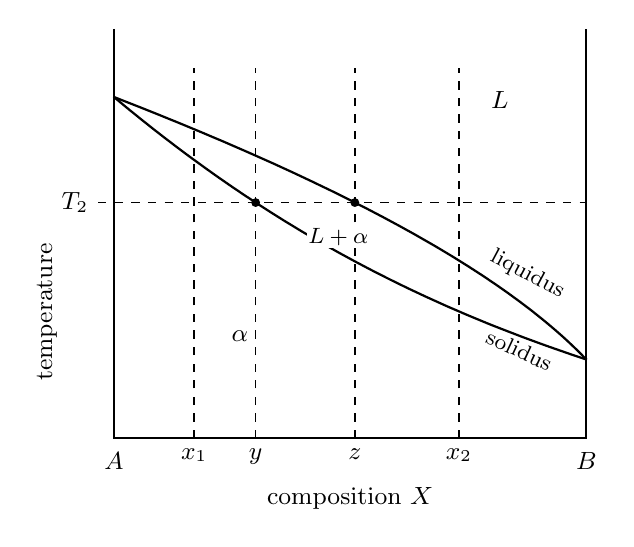
\begin{tikzpicture}[font=\small, >=Latex, line width=0.8pt]
    % frame: pure A on the left, pure B on the right
    \draw (0,5.2) -- (0,0) -- (6,0) -- (6,5.2);
    % liquidus and solidus of ideal solid and liquid solutions (computed)
    \draw plot[smooth] coordinates {(6.000,1.000) (5.999,1.001) (5.944,1.057) (5.888,1.114) (5.829,1.170) (5.769,1.227) (5.708,1.283) (5.644,1.340) (5.579,1.396) (5.513,1.452) (5.444,1.509) (5.374,1.565) (5.303,1.622) (5.229,1.678) (5.154,1.735) (5.077,1.791) (4.999,1.848) (4.919,1.904) (4.837,1.961) (4.754,2.017) (4.669,2.074) (4.582,2.130) (4.494,2.187) (4.404,2.243) (4.313,2.300) (4.220,2.356) (4.125,2.413) (4.029,2.469) (3.931,2.525) (3.832,2.582) (3.731,2.638) (3.628,2.695) (3.524,2.751) (3.418,2.808) (3.311,2.864) (3.202,2.921) (3.092,2.977) (2.980,3.034) (2.867,3.090) (2.752,3.147) (2.635,3.203) (2.517,3.260) (2.398,3.316) (2.277,3.373) (2.155,3.429) (2.031,3.486) (1.905,3.542) (1.779,3.598) (1.650,3.655) (1.521,3.711) (1.390,3.768) (1.257,3.824) (1.123,3.881) (0.988,3.937) (0.851,3.994) (0.713,4.050) (0.573,4.107) (0.433,4.163) (0.290,4.220) (0.147,4.276) (0.002,4.333) (0.000,4.333)};
    \draw plot[smooth] coordinates {(6.000,1.000) (5.998,1.001) (5.829,1.057) (5.665,1.114) (5.505,1.170) (5.348,1.227) (5.196,1.283) (5.048,1.340) (4.903,1.396) (4.761,1.452) (4.623,1.509) (4.488,1.565) (4.356,1.622) (4.226,1.678) (4.100,1.735) (3.976,1.791) (3.854,1.848) (3.735,1.904) (3.618,1.961) (3.504,2.017) (3.391,2.074) (3.281,2.130) (3.172,2.187) (3.066,2.243) (2.961,2.300) (2.858,2.356) (2.757,2.413) (2.657,2.469) (2.559,2.525) (2.463,2.582) (2.367,2.638) (2.274,2.695) (2.181,2.751) (2.090,2.808) (2.001,2.864) (1.912,2.921) (1.825,2.977) (1.739,3.034) (1.653,3.090) (1.569,3.147) (1.486,3.203) (1.404,3.260) (1.323,3.316) (1.243,3.373) (1.164,3.429) (1.086,3.486) (1.008,3.542) (0.932,3.598) (0.856,3.655) (0.781,3.711) (0.707,3.768) (0.633,3.824) (0.560,3.881) (0.488,3.937) (0.417,3.994) (0.346,4.050) (0.276,4.107) (0.206,4.163) (0.137,4.220) (0.069,4.276) (0.001,4.333) (0.000,4.333)};
    % isotherm T_2 and the four compositions
    \draw[dashed, line width=0.6pt] (-0.2,2.993) node[left] {$T_2$} -- (6,2.993);
    \foreach \x/\n in {1.02/x_1, 1.80/y, 3.06/z, 4.38/x_2}
        \draw[dashed, line width=0.6pt] (\x,0) node[below] {$\n$} -- (\x,4.7);
    \fill (1.80,2.993) circle (1.6pt);
    \fill (3.06,2.993) circle (1.6pt);
    % region labels
    \node at (4.9,4.3) {$L$};
    \node at (1.6,1.3) {$\alpha$};
    \node[fill=white, inner sep=0.5pt, font=\footnotesize] at (2.85,2.55) {$L+\alpha$};
    \node[rotate=-28, font=\footnotesize] at (5.25,2.08) {liquidus};
    \node[rotate=-25, font=\footnotesize] at (5.15,1.12) {solidus};
    % axes
    \node[below] at (0,-0.05) {$A$};
    \node[below] at (6,-0.05) {$B$};
    \node[below=14pt] at (3,0) {composition $X$};
    \node[rotate=90] at (-0.85,1.6) {temperature};
\end{tikzpicture}
\end{document}
